\section{ХОД РАБОТЫ}

\subsection{Текст задания}

Для всех вариантов необходимо выполнить следующее:

\begin{itemize}

  \item определить функции в соответствии со своим вариантом задания;
  \item в функции main() реализовать демонстрацию работы созданных функций. Во всех заданиях необходимо использовать функции Win32 API для работы с файлами.

\end{itemize}

В соответствии с восьмым вариантом задания необходимо реализовать функции, представленные на рисунке~\ref{lst:task}. Функция ReadComplex() должна возвращать число фактически прочитанных комплексных чисел.

\begin{lstlisting}[caption=Функции для чтения и записи в файл,label=lst:task]
void WriteComplex(char *fname, struct Complex *buff, int count);
int ReadComplex(char *fname, struct Complex *buff, int count);
\end{lstlisting}

\subsection{Исходные данные}

На рисунке~\ref{lst:struct_and_functions} представлена структура Complex, и ряд функций по работе с комплексными числами, реализованные в предыдущей лабораторной работе.

\begin{lstlisting}[caption=Структура Complex и объявление функций для работы с комплексными числами,label=lst:struct_and_functions]
struct Complex {
  double re;
  double im;
  int error;
};
struct Complex add(struct Complex c1, struct Complex c2);
struct Complex sub(struct Complex c1, struct Complex c2);
struct Complex mul(struct Complex c1, struct Complex c2);
struct Complex div(struct Complex c1, struct Complex c2);
void printComplex(struct Complex c);
\end{lstlisting}

\subsection{Особенности разработанной программы}

В ходе проведения данной лабораторной работы была разработана программа для выполнения арифметических операций над комплексными числами, их чтения из файла, записи в файл, представляющая пользователю консольный интерфейс, защищённый от ошибок некорректного ввода.

Главное меню программы, изображенное на рисунке~\ref{fig:main_menu}, состоит из следующий частей:
\begin{itemize}
  \item отображение двух комплексных чисел, с которыми предполагается выполнение арифметических операций;
  \item изменение комплексных чисел;
  \item арифметические операции над комплексными числами;
  \item чтение и запись из файла;
  \item завершение работы с программой.
\end{itemize}

\begin{figure}[htbp]
  \centering
  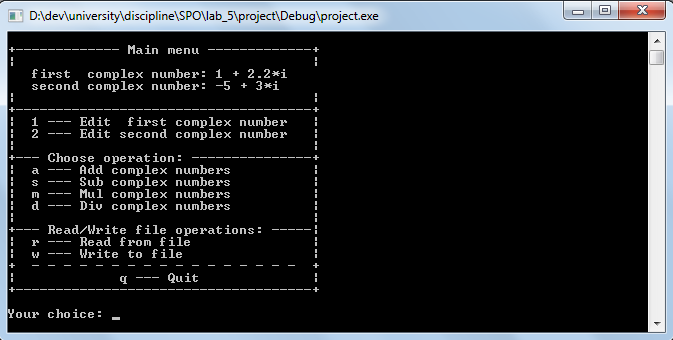
\includegraphics[width=150mm,height=80mm]{img/main_menu}
  \caption{Главное меню программы}\label{fig:main_menu}
\end{figure}


Для того, чтобы записать комплексные числа в файл пользователь должен перейти в пункт меню <<Write to file>>. Далее есть возможность изменить, добавить или удалить числа для записи. Данное меню представлено на рисунке~\ref{fig:write_menu}. После того, как пользователя устроит содержание и количество записываемых чисел, он выбирает пункт меню <<Write complex number>>.

\begin{figure}[htbp]
  \centering
  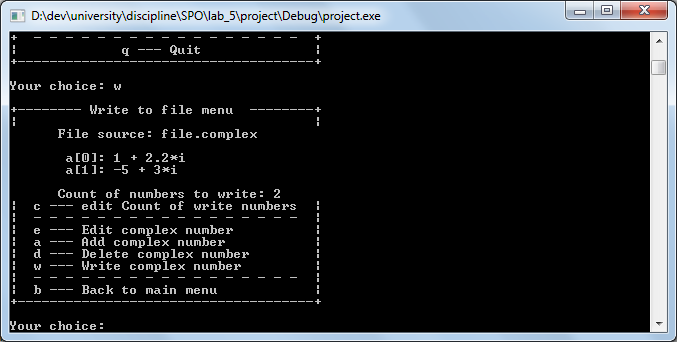
\includegraphics[width=150mm,height=80mm]{img/write_menu}
  \caption{Меню записи комплексных чисел в файл}\label{fig:write_menu}
\end{figure}

Как только запись будет завершена, в командную строку будет выведено сообщение о результате работы вызываемой функции.

Пользователю также доступно подменю чтения комплексных чисел из файла, представленное на рисунке~\ref{fig:read_menu}.

\begin{figure}[htbp]
  \centering
  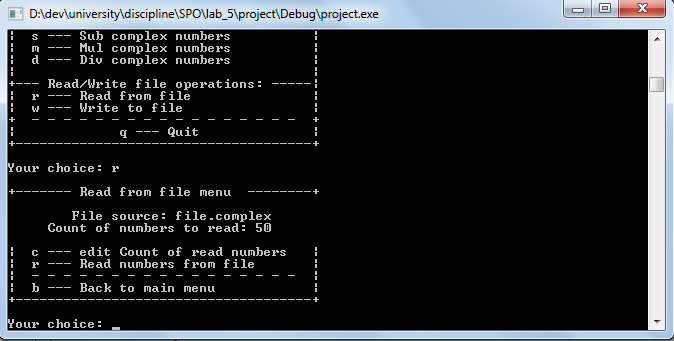
\includegraphics[width=150mm,height=80mm]{img/read_menu}
  \caption{Меню чтения комплексных чисел из файла}\label{fig:read_menu}
\end{figure}

 Имеется возможность изменить количество комплексных чисел для чтения, прочитать данные из файла или вернуться в главное меню. В случае, если количество заданных пользователем чисел для чтения значительно превысит число фактически прочитанных элементов, программа высвободит не используемую программой память.

Пример работы функции чтения комплексных чисел из файла представлен на рисунке~\ref{fig:read_results}.

\begin{figure}[htbp]
  \centering
  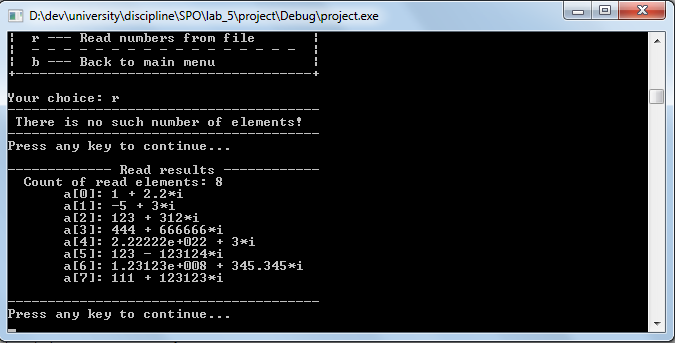
\includegraphics[width=150mm,height=80mm]{img/read_results}
  \caption{Результат чтения комплексных чисел из файла}\label{fig:read_results}
\end{figure}

Исходный текст разработанной программы расположен в приложении~А.

\newpage